% Figure of the starter poster (scripts/gen-starters.ts compiles it to templates/starters/poster/figures/model.pdf).
\documentclass[border=4pt]{standalone}
\usepackage[T1]{fontenc}
\usepackage[scaled]{helvet}
\renewcommand{\familydefault}{\sfdefault}
\usepackage{sansmath}
\usepackage{tikz}
\usetikzlibrary{arrows.meta,positioning}
\definecolor{jblue}{RGB}{31,78,140}
\begin{document}
\sansmath
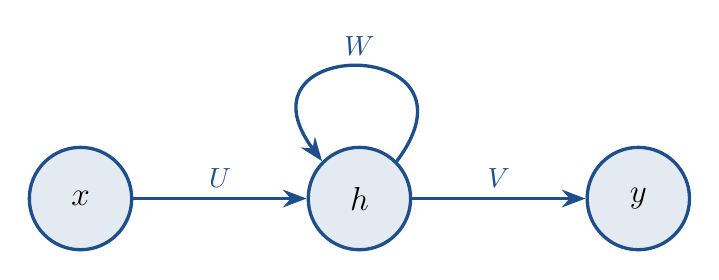
\begin{tikzpicture}[node distance=2.2cm, >={Stealth[length=3mm]}, line width=1.2pt,
  unit/.style={circle, draw=jblue, fill=jblue!12, minimum size=1.3cm, font=\large}]
\node[unit] (x) {$x$};
\node[unit, right=of x] (h) {$h$};
\node[unit, right=of h] (y) {$y$};
\draw[->, jblue] (x) -- node[above] {$U$} (h);
\draw[->, jblue] (h) -- node[above] {$V$} (y);
\draw[->, jblue] (h.north east) .. controls +(1.2,1.6) and +(-1.2,1.6) .. node[above] {$W$} (h.north west);
\end{tikzpicture}
\end{document}
